\subsection{Example: $\Vec(\Z/2)$ spin chain}

We consider a one-dimensional spin chain of $N$ particles, i.e., a chain
	\begin{figure}[H]
		
\begin{tikzpicture}[scale=1.5]
			\fill[black] (0,0) circle (0.07cm);
			\fill[black] (0.5,0) circle (0.07cm);
			\fill[black] (1,0) circle (0.07cm);
			\fill[black] (1.5,0) circle (0.07cm);
			\fill[black] (2,0) circle (0.07cm);
			\fill[black] (2.5,0) circle (0.07cm);
			\fill[black] (3,0) circle (0.07cm);
			\fill[black] (4,0) circle (0.07cm);
			\node at (3.5,0) {$\dots$};
		\end{tikzpicture}
	\end{figure}
\noindent
whose Hilbert space is 
	\begin{equation}
		\mathcal{H}_0=\bigotimes_{i=1}^N \mathbb{C}^2.
	\end{equation}
We now introduce defects, which means that one of the spins, say the spin at site $j$, is replaced by a different kind of spin, e.g., no spin (indicated in red): 
	\begin{figure}[H]
		
\begin{tikzpicture}[scale=1.5]
			\fill[black] (0,0) circle (0.07cm);
			\fill[black] (0.5,0) circle (0.07cm);
			\fill[black] (1,0) circle (0.07cm);
			\fill[black] (1.5,0) circle (0.07cm);
			\fill[red] (2,0) circle (0.07cm);
			\fill[black] (2.5,0) circle (0.07cm);
			\fill[black] (3,0) circle (0.07cm);
			\fill[black] (4,0) circle (0.07cm);
			\node at (3.5,0) {$\dots$};
		\end{tikzpicture}
	\end{figure}
\noindent
This corresponds to replacing the Hilbert space $\mathbb{C}^2$ at site $j$ with $\mathbb{C}$, which results in the overall Hilbert space
	\begin{equation}
		\mathcal{H}_1^{(j)}=\left(\bigotimes_{i=1}^{j-1}\mathbb{C}^2\right)\otimes\mathbb{C}\otimes\left(\bigotimes_{i=j+1}^N\mathbb{C}^2\right).
	\end{equation}
The subscript here denotes the number of defects in the chain and the superscript indicates at which site the defect appears. If we want to consider both possibilities, having no defect and having a defect at site $j$, we use the Hilbert space
	\begin{equation}
		\mathcal{H}=\mathcal{H}_0\oplus\mathcal{H}_1^{(j)}.
	\end{equation}
We can also allow the defect to move, which means still restrict the setting to only one defect in total, but it can happen at any site. Hence, the overall Hilbert space becomes
	\begin{equation}
		\mathcal{H}=\mathcal{H}_0\oplus\left(\bigoplus_{j=1}^N\mathcal{H}_1^{(j)}\right).
	\end{equation}
We can generalize this construction to an arbitrary number of defects: The Hilbert space for having defects at sites $j$ and $k$ is 
	\begin{equation}
		\mathcal{H}_2^{(j,k)}=\left(\bigotimes_{i=1}^{j-1}\mathbb{C}^2\right)\otimes\mathbb{C}\otimes\left(\bigotimes_{i=j+1}^{k-1}\mathbb{C}^2\right)\otimes\mathbb{C}\otimes\left(\bigotimes_{i=k+1}^{N}\mathbb{C}^2\right).
	\end{equation}
Again, if we allow these defects to move and also include the possibilities of having only one defect and no defect at all, the overall Hilbert space is
	\begin{equation}
		\mathcal{H}=\mathcal{H}_0\oplus\left(\bigoplus_{j=1}^N\mathcal{H}_1^{(j)}\right)\oplus\left(\bigoplus_{j=1}^N\bigoplus_{k\neq j}\mathcal{H}_2^{(j,k)}\right).
	\end{equation}
We can continue this construction until we have a defect at every site of the chain, i.e.
	\begin{equation}
		\mathcal{H}_N=\bigotimes_{i=1}^N\mathbb{C},
	\end{equation}
and the overall Hilbert space is then
	\begin{equation}
		\mathcal{H}=\bigoplus_{n\in\#\mathrm{defects}}\mathcal{H}_n,
	\end{equation}
where $\mathcal{H}_n$ is the direct sum of all possible Hilbert spaces with $n$ defects, as constructed above. Since this is now a very complicated Hilbert space, we can also think about it in a different and simpler way: at each site, the particle can be in one of three states: spin up, spin down, or no spin. Hence, we have effectively a three-level system at each site of the chain, and therefore the overall Hilbert space can be written as
	\begin{equation}
		\mathcal{H}\cong\bigotimes_{j=1}^N\left(\mathbb{C}\oplus\mathbb{C}^2\right).
	\end{equation}

We will now look at the example of a particle chain with $\Vec(\Z/2)$ fusion rules, i.e.\ the objects are either $0$ or $1$ and the fusion is given by addition $\mathrm{mod}\ 2$. We consider the following chain:
	\begin{figure}[H]
		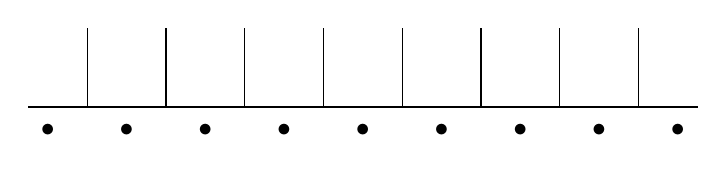
\begin{tikzpicture}
			\draw (-0.25,0) -- (8.25,0);
			\draw (0.5,0) -- (0.5,1);
			\draw (1.5,0) -- (1.5,1);
			\draw (2.5,0) -- (2.5,1);
			\draw (3.5,0) -- (3.5,1);
			\draw (4.5,0) -- (4.5,1);
			\draw (5.5,0) -- (5.5,1);
			\draw (6.5,0) -- (6.5,1);
			\draw (7.5,0) -- (7.5,1);
			\node at (0,-0.3) {$\bullet$};
			\node at (1,-0.3) {$\bullet$};
			\node at (2,-0.3) {$\bullet$};
			\node at (3,-0.3) {$\bullet$};
			\node at (4,-0.3) {$\bullet$};
			\node at (5,-0.3) {$\bullet$};
			\node at (6,-0.3) {$\bullet$};
			\node at (7,-0.3) {$\bullet$};
			\node at (8,-0.3) {$\bullet$};
		\end{tikzpicture}
	\end{figure}
\noindent
where the bullets can either be $0$ or $1$ (according to the fusion rules), hence they represent the space $\mathbb{C}^2$.
If we only fuse $1$-particles to the chain, we get
	\begin{figure}[H]
		\begin{tikzpicture}
			\draw (-0.25,0) -- (8.25,0);
			\draw (0.5,0) -- (0.5,1);
			\draw (1.5,0) -- (1.5,1);
			\draw (2.5,0) -- (2.5,1);
			\draw (3.5,0) -- (3.5,1);
			\draw (4.5,0) -- (4.5,1);
			\draw (5.5,0) -- (5.5,1);
			\draw (6.5,0) -- (6.5,1);
			\draw (7.5,0) -- (7.5,1);
			\node at (0.5,1.3) {$1$};
			\node at (1.5,1.3) {$1$};
			\node at (2.5,1.3) {$1$};
			\node at (3.5,1.3) {$1$};
			\node at (4.5,1.3) {$1$};
			\node at (5.5,1.3) {$1$};
			\node at (6.5,1.3) {$1$};
			\node at (7.5,1.3) {$1$};
			\node at (0,-0.3) {$\bullet$};
			\node at (1,-0.3) {$\bullet$};
			\node at (2,-0.3) {$\bullet$};
			\node at (3,-0.3) {$\bullet$};
			\node at (4,-0.3) {$\bullet$};
			\node at (5,-0.3) {$\bullet$};
			\node at (6,-0.3) {$\bullet$};
			\node at (7,-0.3) {$\bullet$};
			\node at (8,-0.3) {$\bullet$};
		\end{tikzpicture}
	\end{figure}
\noindent
Now, the value of the bullets is fixed by the fusion rules: When we fix the outer labels (e.g., to $1$), the only possible labelling is
	\begin{figure}[H]
		\begin{tikzpicture}
			\draw (-0.25,0) -- (8.25,0);
			\draw (0.5,0) -- (0.5,1);
			\draw (1.5,0) -- (1.5,1);
			\draw (2.5,0) -- (2.5,1);
			\draw (3.5,0) -- (3.5,1);
			\draw (4.5,0) -- (4.5,1);
			\draw (5.5,0) -- (5.5,1);
			\draw (6.5,0) -- (6.5,1);
			\draw (7.5,0) -- (7.5,1);
			\node at (0.5,1.3) {$1$};
			\node at (1.5,1.3) {$1$};
			\node at (2.5,1.3) {$1$};
			\node at (3.5,1.3) {$1$};
			\node at (4.5,1.3) {$1$};
			\node at (5.5,1.3) {$1$};
			\node at (6.5,1.3) {$1$};
			\node at (7.5,1.3) {$1$};
			\node at (0,-0.3) {$1$};
			\node at (1,-0.3) {$0$};
			\node at (2,-0.3) {$1$};
			\node at (3,-0.3) {$0$};
			\node at (4,-0.3) {$1$};
			\node at (5,-0.3) {$0$};
			\node at (6,-0.3) {$1$};
			\node at (7,-0.3) {$0$};
			\node at (8,-0.3) {$1$};
		\end{tikzpicture}
	\end{figure}
\noindent
Hence, we have a unique ground state and the only vertices occurring in this case are
	\begin{figure}[H]	
		\begin{tikzpicture}
			\draw (0,0) -- (1.5,0);
			\draw (0.75,0) -- (0.75,1);
			\node at (0,-0.3) {$0$};
			\node at (1.5,-0.3) {$1$};
			\node at (0.75,1.3) {$1$};
		\end{tikzpicture}
		\hspace{20pt}
		\begin{tikzpicture}
			\draw (0,0) -- (1.5,0);
			\draw (0.75,0) -- (0.75,1);
			\node at (0,-0.3) {$1$};
			\node at (1.5,-0.3) {$0$};
			\node at (0.75,1.3) {$1$};
		\end{tikzpicture}
	\end{figure}
\noindent
Analogously, if we only allow $0$s to fuse to the chain, the bullets are either all $0$ or all $1$, which means we have the vertices
	\begin{figure}[H]	
		\begin{tikzpicture}
		\draw (0,0) -- (1.5,0);
		\draw (0.75,0) -- (0.75,1);
		\node at (0,-0.3) {$0$};
		\node at (1.5,-0.3) {$0$};
		\node at (0.75,1.3) {$0$};
		\end{tikzpicture}
		\hspace{20pt}
		\begin{tikzpicture}
		\draw (0,0) -- (1.5,0);
		\draw (0.75,0) -- (0.75,1);
		\node at (0,-0.3) {$1$};
		\node at (1.5,-0.3) {$1$};
		\node at (0.75,1.3) {$0$};
		\end{tikzpicture}
	\end{figure}
\noindent
Hence, in the case of open boundary conditions, the chain has a \emph{unique ground state} once we fix the outer labels of the chain. The situation is different for periodic boundary conditions: since the only requirement here is that the label at site $n+1$ has to equal the label at site $1$, there are two possibilities of labelling the chain. For instance, in the case of only fusing $1$s to the chain, the two possibilities are
	\begin{figure}[H]
		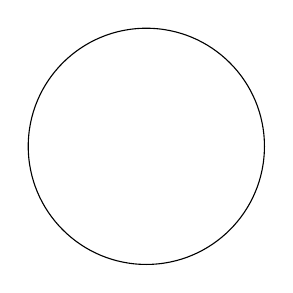
\begin{tikzpicture}
			\def\Radius{1.5cm}
			\draw (0,0) circle[radius=\Radius];
		\end{tikzpicture}
		\hspace{40pt}
		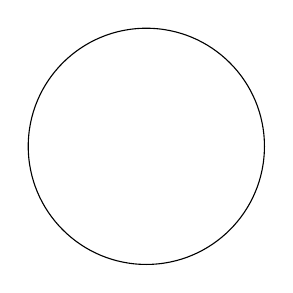
\begin{tikzpicture}
			\def\Radius{1.5cm}
			\draw (0,0) circle[radius=\Radius];
		\end{tikzpicture}
	\end{figure}